% Created by tikzDevice version 0.12 on 2019-03-04 16:30:39
% !TEX encoding = UTF-8 Unicode
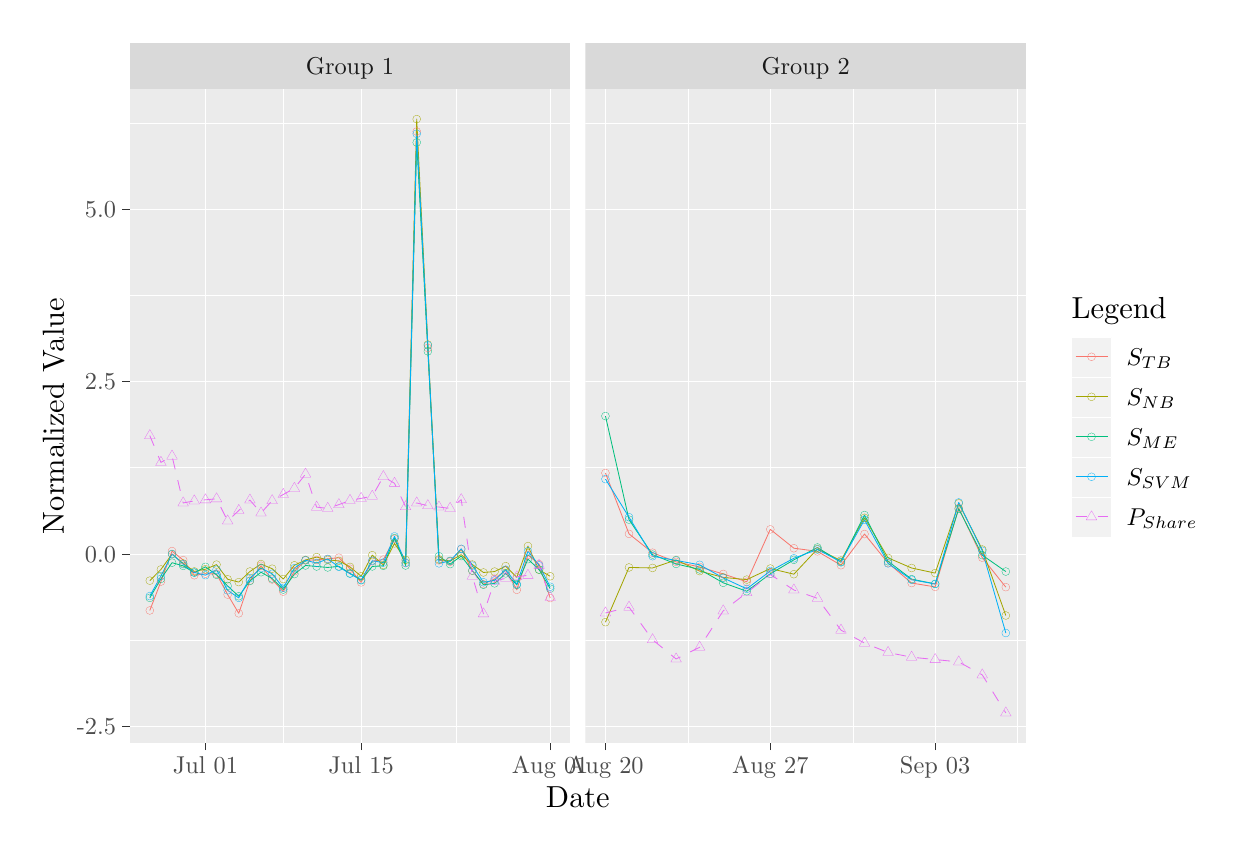
\begin{tikzpicture}[x=1pt,y=1pt]
\definecolor{fillColor}{RGB}{255,255,255}
\path[use as bounding box,fill=fillColor,fill opacity=0.00] (0,0) rectangle (433.62,289.08);
\begin{scope}
\path[clip] (  0.00,  0.00) rectangle (433.62,289.08);
\definecolor{drawColor}{RGB}{255,255,255}
\definecolor{fillColor}{RGB}{255,255,255}

\path[draw=drawColor,line width= 0.1pt,line join=round,line cap=round,fill=fillColor] (  0.00,  0.00) rectangle (433.62,289.08);
\end{scope}
\begin{scope}
\path[clip] ( 36.90, 30.73) rectangle (196.04,266.77);
\definecolor{fillColor}{gray}{0.92}

\path[fill=fillColor] ( 36.90, 30.73) rectangle (196.04,266.77);
\definecolor{drawColor}{RGB}{255,255,255}

\path[draw=drawColor,line width= 0.1pt,line join=round] ( 36.90, 67.88) --
	(196.04, 67.88);

\path[draw=drawColor,line width= 0.1pt,line join=round] ( 36.90,130.12) --
	(196.04,130.12);

\path[draw=drawColor,line width= 0.1pt,line join=round] ( 36.90,192.37) --
	(196.04,192.37);

\path[draw=drawColor,line width= 0.1pt,line join=round] ( 36.90,254.62) --
	(196.04,254.62);

\path[draw=drawColor,line width= 0.1pt,line join=round] ( 92.36, 30.73) --
	( 92.36,266.77);

\path[draw=drawColor,line width= 0.1pt,line join=round] (154.65, 30.73) --
	(154.65,266.77);

\path[draw=drawColor,line width= 0.1pt,line join=round] ( 36.90, 36.76) --
	(196.04, 36.76);

\path[draw=drawColor,line width= 0.1pt,line join=round] ( 36.90, 99.00) --
	(196.04, 99.00);

\path[draw=drawColor,line width= 0.1pt,line join=round] ( 36.90,161.25) --
	(196.04,161.25);

\path[draw=drawColor,line width= 0.1pt,line join=round] ( 36.90,223.49) --
	(196.04,223.49);

\path[draw=drawColor,line width= 0.1pt,line join=round] ( 64.23, 30.73) --
	( 64.23,266.77);

\path[draw=drawColor,line width= 0.1pt,line join=round] (120.49, 30.73) --
	(120.49,266.77);

\path[draw=drawColor,line width= 0.1pt,line join=round] (188.81, 30.73) --
	(188.81,266.77);
\definecolor{drawColor}{RGB}{248,118,109}

\path[draw=drawColor,line width= 0.3pt,line join=round] ( 44.13, 78.49) --
	( 48.15, 88.93) --
	( 52.17, 99.95) --
	( 56.19, 96.70) --
	( 60.21, 91.22) --
	( 64.23, 91.75) --
	( 68.25, 91.69) --
	( 72.26, 84.22) --
	( 76.28, 77.45) --
	( 80.30, 89.28) --
	( 84.32, 94.64) --
	( 88.34, 89.68) --
	( 92.36, 85.29) --
	( 96.38, 92.68) --
	(100.40, 96.62) --
	(104.42, 96.77) --
	(108.43, 97.14) --
	(112.45, 97.55) --
	(116.47, 93.56) --
	(120.49, 88.63) --
	(124.51, 96.29) --
	(128.53, 96.87) --
	(132.55,104.37) --
	(136.57, 95.60) --
	(140.58,251.55) --
	(144.60,173.35) --
	(148.62, 96.60) --
	(152.64, 96.12) --
	(156.66,100.63) --
	(160.68, 92.82) --
	(164.70, 87.97) --
	(168.72, 89.92) --
	(172.73, 93.03) --
	(176.75, 85.94) --
	(180.77, 98.54) --
	(184.79, 95.22) --
	(188.81, 82.98);
\definecolor{drawColor}{RGB}{163,165,0}

\path[draw=drawColor,line width= 0.3pt,line join=round] ( 44.13, 89.26) --
	( 48.15, 93.31) --
	( 52.17, 98.83) --
	( 56.19, 95.46) --
	( 60.21, 92.59) --
	( 64.23, 93.40) --
	( 68.25, 95.06) --
	( 72.26, 89.76) --
	( 76.28, 88.74) --
	( 80.30, 92.57) --
	( 84.32, 95.26) --
	( 88.34, 93.57) --
	( 92.36, 89.85) --
	( 96.38, 94.81) --
	(100.40, 96.74) --
	(104.42, 97.77) --
	(108.43, 96.74) --
	(112.45, 96.42) --
	(116.47, 94.23) --
	(120.49, 90.86) --
	(124.51, 98.48) --
	(128.53, 94.93) --
	(132.55,102.72) --
	(136.57, 96.77) --
	(140.58,256.04) --
	(144.60,174.57) --
	(148.62, 96.95) --
	(152.64, 96.37) --
	(156.66, 98.66) --
	(160.68, 95.08) --
	(164.70, 92.22) --
	(168.72, 92.54) --
	(172.73, 94.51) --
	(176.75, 90.44) --
	(180.77,101.76) --
	(184.79, 93.17) --
	(188.81, 90.85);
\definecolor{drawColor}{RGB}{0,191,125}

\path[draw=drawColor,line width= 0.3pt,line join=round] ( 44.13, 83.03) --
	( 48.15, 89.91) --
	( 52.17, 95.75) --
	( 56.19, 94.60) --
	( 60.21, 92.13) --
	( 64.23, 94.25) --
	( 68.25, 91.36) --
	( 72.26, 87.33) --
	( 76.28, 83.63) --
	( 80.30, 89.13) --
	( 84.32, 92.31) --
	( 88.34, 90.03) --
	( 92.36, 86.05) --
	( 96.38, 91.64) --
	(100.40, 94.74) --
	(104.42, 94.38) --
	(108.43, 94.03) --
	(112.45, 94.42) --
	(116.47, 91.91) --
	(120.49, 89.42) --
	(124.51, 94.40) --
	(128.53, 94.61) --
	(132.55,104.63) --
	(136.57, 94.74) --
	(140.58,247.60) --
	(144.60,172.13) --
	(148.62, 98.10) --
	(152.64, 95.24) --
	(156.66, 98.15) --
	(160.68, 92.91) --
	(164.70, 87.76) --
	(168.72, 88.28) --
	(172.73, 91.88) --
	(176.75, 87.70) --
	(180.77, 97.03) --
	(184.79, 93.29) --
	(188.81, 86.37);
\definecolor{drawColor}{RGB}{0,176,246}

\path[draw=drawColor,line width= 0.3pt,line join=round] ( 44.13, 83.69) --
	( 48.15, 90.92) --
	( 52.17, 98.91) --
	( 56.19, 95.23) --
	( 60.21, 92.23) --
	( 64.23, 91.24) --
	( 68.25, 93.21) --
	( 72.26, 85.76) --
	( 76.28, 83.04) --
	( 80.30, 90.15) --
	( 84.32, 93.79) --
	( 88.34, 91.75) --
	( 92.36, 86.64) --
	( 96.38, 93.77) --
	(100.40, 96.61) --
	(104.42, 95.63) --
	(108.43, 97.08) --
	(112.45, 94.25) --
	(116.47, 91.75) --
	(120.49, 89.56) --
	(124.51, 96.43) --
	(128.53, 95.79) --
	(132.55,105.27) --
	(136.57, 95.71) --
	(140.58,250.74) --
	(144.60,174.30) --
	(148.62, 95.50) --
	(152.64, 96.39) --
	(156.66,100.76) --
	(160.68, 94.68) --
	(164.70, 88.68) --
	(168.72, 89.35) --
	(172.73, 93.21) --
	(176.75, 87.97) --
	(180.77, 99.89) --
	(184.79, 94.80) --
	(188.81, 87.05);
\definecolor{drawColor}{RGB}{231,107,243}

\path[draw=drawColor,line width= 0.3pt,dash pattern=on 4pt off 4pt ,line join=round] ( 44.13,141.67) --
	( 48.15,131.99) --
	( 52.17,134.26) --
	( 56.19,117.33) --
	( 60.21,118.09) --
	( 64.23,118.47) --
	( 68.25,118.84) --
	( 72.26,110.83) --
	( 76.28,114.61) --
	( 80.30,118.39) --
	( 84.32,113.71) --
	( 88.34,118.16) --
	( 92.36,120.39) --
	( 96.38,122.62) --
	(100.40,127.76) --
	(104.42,115.82) --
	(108.43,115.37) --
	(112.45,116.73) --
	(116.47,118.24) --
	(120.49,119.00) --
	(124.51,119.75) --
	(128.53,126.85) --
	(132.55,124.44) --
	(136.57,115.97) --
	(140.58,117.33) --
	(144.60,116.35) --
	(148.62,115.86) --
	(152.64,115.37) --
	(156.66,118.54) --
	(160.68, 90.88) --
	(164.70, 77.28) --
	(168.72, 89.07) --
	(172.73, 90.13) --
	(176.75, 90.66) --
	(180.77, 91.18) --
	(184.79, 94.81) --
	(188.81, 83.17);
\definecolor{drawColor}{RGB}{248,118,109}

\path[draw=drawColor,line width= 0.1pt,line join=round,line cap=round] ( 44.13, 78.49) circle (  1.43);

\path[draw=drawColor,line width= 0.1pt,line join=round,line cap=round] ( 48.15, 88.93) circle (  1.43);

\path[draw=drawColor,line width= 0.1pt,line join=round,line cap=round] ( 52.17, 99.95) circle (  1.43);

\path[draw=drawColor,line width= 0.1pt,line join=round,line cap=round] ( 56.19, 96.70) circle (  1.43);

\path[draw=drawColor,line width= 0.1pt,line join=round,line cap=round] ( 60.21, 91.22) circle (  1.43);

\path[draw=drawColor,line width= 0.1pt,line join=round,line cap=round] ( 64.23, 91.75) circle (  1.43);

\path[draw=drawColor,line width= 0.1pt,line join=round,line cap=round] ( 68.25, 91.69) circle (  1.43);

\path[draw=drawColor,line width= 0.1pt,line join=round,line cap=round] ( 72.26, 84.22) circle (  1.43);

\path[draw=drawColor,line width= 0.1pt,line join=round,line cap=round] ( 76.28, 77.45) circle (  1.43);

\path[draw=drawColor,line width= 0.1pt,line join=round,line cap=round] ( 80.30, 89.28) circle (  1.43);

\path[draw=drawColor,line width= 0.1pt,line join=round,line cap=round] ( 84.32, 94.64) circle (  1.43);

\path[draw=drawColor,line width= 0.1pt,line join=round,line cap=round] ( 88.34, 89.68) circle (  1.43);

\path[draw=drawColor,line width= 0.1pt,line join=round,line cap=round] ( 92.36, 85.29) circle (  1.43);

\path[draw=drawColor,line width= 0.1pt,line join=round,line cap=round] ( 96.38, 92.68) circle (  1.43);

\path[draw=drawColor,line width= 0.1pt,line join=round,line cap=round] (100.40, 96.62) circle (  1.43);

\path[draw=drawColor,line width= 0.1pt,line join=round,line cap=round] (104.42, 96.77) circle (  1.43);

\path[draw=drawColor,line width= 0.1pt,line join=round,line cap=round] (108.43, 97.14) circle (  1.43);

\path[draw=drawColor,line width= 0.1pt,line join=round,line cap=round] (112.45, 97.55) circle (  1.43);

\path[draw=drawColor,line width= 0.1pt,line join=round,line cap=round] (116.47, 93.56) circle (  1.43);

\path[draw=drawColor,line width= 0.1pt,line join=round,line cap=round] (120.49, 88.63) circle (  1.43);

\path[draw=drawColor,line width= 0.1pt,line join=round,line cap=round] (124.51, 96.29) circle (  1.43);

\path[draw=drawColor,line width= 0.1pt,line join=round,line cap=round] (128.53, 96.87) circle (  1.43);

\path[draw=drawColor,line width= 0.1pt,line join=round,line cap=round] (132.55,104.37) circle (  1.43);

\path[draw=drawColor,line width= 0.1pt,line join=round,line cap=round] (136.57, 95.60) circle (  1.43);

\path[draw=drawColor,line width= 0.1pt,line join=round,line cap=round] (140.58,251.55) circle (  1.43);

\path[draw=drawColor,line width= 0.1pt,line join=round,line cap=round] (144.60,173.35) circle (  1.43);

\path[draw=drawColor,line width= 0.1pt,line join=round,line cap=round] (148.62, 96.60) circle (  1.43);

\path[draw=drawColor,line width= 0.1pt,line join=round,line cap=round] (152.64, 96.12) circle (  1.43);

\path[draw=drawColor,line width= 0.1pt,line join=round,line cap=round] (156.66,100.63) circle (  1.43);

\path[draw=drawColor,line width= 0.1pt,line join=round,line cap=round] (160.68, 92.82) circle (  1.43);

\path[draw=drawColor,line width= 0.1pt,line join=round,line cap=round] (164.70, 87.97) circle (  1.43);

\path[draw=drawColor,line width= 0.1pt,line join=round,line cap=round] (168.72, 89.92) circle (  1.43);

\path[draw=drawColor,line width= 0.1pt,line join=round,line cap=round] (172.73, 93.03) circle (  1.43);

\path[draw=drawColor,line width= 0.1pt,line join=round,line cap=round] (176.75, 85.94) circle (  1.43);

\path[draw=drawColor,line width= 0.1pt,line join=round,line cap=round] (180.77, 98.54) circle (  1.43);

\path[draw=drawColor,line width= 0.1pt,line join=round,line cap=round] (184.79, 95.22) circle (  1.43);

\path[draw=drawColor,line width= 0.1pt,line join=round,line cap=round] (188.81, 82.98) circle (  1.43);
\definecolor{drawColor}{RGB}{163,165,0}

\path[draw=drawColor,line width= 0.1pt,line join=round,line cap=round] ( 44.13, 89.26) circle (  1.43);

\path[draw=drawColor,line width= 0.1pt,line join=round,line cap=round] ( 48.15, 93.31) circle (  1.43);

\path[draw=drawColor,line width= 0.1pt,line join=round,line cap=round] ( 52.17, 98.83) circle (  1.43);

\path[draw=drawColor,line width= 0.1pt,line join=round,line cap=round] ( 56.19, 95.46) circle (  1.43);

\path[draw=drawColor,line width= 0.1pt,line join=round,line cap=round] ( 60.21, 92.59) circle (  1.43);

\path[draw=drawColor,line width= 0.1pt,line join=round,line cap=round] ( 64.23, 93.40) circle (  1.43);

\path[draw=drawColor,line width= 0.1pt,line join=round,line cap=round] ( 68.25, 95.06) circle (  1.43);

\path[draw=drawColor,line width= 0.1pt,line join=round,line cap=round] ( 72.26, 89.76) circle (  1.43);

\path[draw=drawColor,line width= 0.1pt,line join=round,line cap=round] ( 76.28, 88.74) circle (  1.43);

\path[draw=drawColor,line width= 0.1pt,line join=round,line cap=round] ( 80.30, 92.57) circle (  1.43);

\path[draw=drawColor,line width= 0.1pt,line join=round,line cap=round] ( 84.32, 95.26) circle (  1.43);

\path[draw=drawColor,line width= 0.1pt,line join=round,line cap=round] ( 88.34, 93.57) circle (  1.43);

\path[draw=drawColor,line width= 0.1pt,line join=round,line cap=round] ( 92.36, 89.85) circle (  1.43);

\path[draw=drawColor,line width= 0.1pt,line join=round,line cap=round] ( 96.38, 94.81) circle (  1.43);

\path[draw=drawColor,line width= 0.1pt,line join=round,line cap=round] (100.40, 96.74) circle (  1.43);

\path[draw=drawColor,line width= 0.1pt,line join=round,line cap=round] (104.42, 97.77) circle (  1.43);

\path[draw=drawColor,line width= 0.1pt,line join=round,line cap=round] (108.43, 96.74) circle (  1.43);

\path[draw=drawColor,line width= 0.1pt,line join=round,line cap=round] (112.45, 96.42) circle (  1.43);

\path[draw=drawColor,line width= 0.1pt,line join=round,line cap=round] (116.47, 94.23) circle (  1.43);

\path[draw=drawColor,line width= 0.1pt,line join=round,line cap=round] (120.49, 90.86) circle (  1.43);

\path[draw=drawColor,line width= 0.1pt,line join=round,line cap=round] (124.51, 98.48) circle (  1.43);

\path[draw=drawColor,line width= 0.1pt,line join=round,line cap=round] (128.53, 94.93) circle (  1.43);

\path[draw=drawColor,line width= 0.1pt,line join=round,line cap=round] (132.55,102.72) circle (  1.43);

\path[draw=drawColor,line width= 0.1pt,line join=round,line cap=round] (136.57, 96.77) circle (  1.43);

\path[draw=drawColor,line width= 0.1pt,line join=round,line cap=round] (140.58,256.04) circle (  1.43);

\path[draw=drawColor,line width= 0.1pt,line join=round,line cap=round] (144.60,174.57) circle (  1.43);

\path[draw=drawColor,line width= 0.1pt,line join=round,line cap=round] (148.62, 96.95) circle (  1.43);

\path[draw=drawColor,line width= 0.1pt,line join=round,line cap=round] (152.64, 96.37) circle (  1.43);

\path[draw=drawColor,line width= 0.1pt,line join=round,line cap=round] (156.66, 98.66) circle (  1.43);

\path[draw=drawColor,line width= 0.1pt,line join=round,line cap=round] (160.68, 95.08) circle (  1.43);

\path[draw=drawColor,line width= 0.1pt,line join=round,line cap=round] (164.70, 92.22) circle (  1.43);

\path[draw=drawColor,line width= 0.1pt,line join=round,line cap=round] (168.72, 92.54) circle (  1.43);

\path[draw=drawColor,line width= 0.1pt,line join=round,line cap=round] (172.73, 94.51) circle (  1.43);

\path[draw=drawColor,line width= 0.1pt,line join=round,line cap=round] (176.75, 90.44) circle (  1.43);

\path[draw=drawColor,line width= 0.1pt,line join=round,line cap=round] (180.77,101.76) circle (  1.43);

\path[draw=drawColor,line width= 0.1pt,line join=round,line cap=round] (184.79, 93.17) circle (  1.43);

\path[draw=drawColor,line width= 0.1pt,line join=round,line cap=round] (188.81, 90.85) circle (  1.43);
\definecolor{drawColor}{RGB}{0,191,125}

\path[draw=drawColor,line width= 0.1pt,line join=round,line cap=round] ( 44.13, 83.03) circle (  1.43);

\path[draw=drawColor,line width= 0.1pt,line join=round,line cap=round] ( 48.15, 89.91) circle (  1.43);

\path[draw=drawColor,line width= 0.1pt,line join=round,line cap=round] ( 52.17, 95.75) circle (  1.43);

\path[draw=drawColor,line width= 0.1pt,line join=round,line cap=round] ( 56.19, 94.60) circle (  1.43);

\path[draw=drawColor,line width= 0.1pt,line join=round,line cap=round] ( 60.21, 92.13) circle (  1.43);

\path[draw=drawColor,line width= 0.1pt,line join=round,line cap=round] ( 64.23, 94.25) circle (  1.43);

\path[draw=drawColor,line width= 0.1pt,line join=round,line cap=round] ( 68.25, 91.36) circle (  1.43);

\path[draw=drawColor,line width= 0.1pt,line join=round,line cap=round] ( 72.26, 87.33) circle (  1.43);

\path[draw=drawColor,line width= 0.1pt,line join=round,line cap=round] ( 76.28, 83.63) circle (  1.43);

\path[draw=drawColor,line width= 0.1pt,line join=round,line cap=round] ( 80.30, 89.13) circle (  1.43);

\path[draw=drawColor,line width= 0.1pt,line join=round,line cap=round] ( 84.32, 92.31) circle (  1.43);

\path[draw=drawColor,line width= 0.1pt,line join=round,line cap=round] ( 88.34, 90.03) circle (  1.43);

\path[draw=drawColor,line width= 0.1pt,line join=round,line cap=round] ( 92.36, 86.05) circle (  1.43);

\path[draw=drawColor,line width= 0.1pt,line join=round,line cap=round] ( 96.38, 91.64) circle (  1.43);

\path[draw=drawColor,line width= 0.1pt,line join=round,line cap=round] (100.40, 94.74) circle (  1.43);

\path[draw=drawColor,line width= 0.1pt,line join=round,line cap=round] (104.42, 94.38) circle (  1.43);

\path[draw=drawColor,line width= 0.1pt,line join=round,line cap=round] (108.43, 94.03) circle (  1.43);

\path[draw=drawColor,line width= 0.1pt,line join=round,line cap=round] (112.45, 94.42) circle (  1.43);

\path[draw=drawColor,line width= 0.1pt,line join=round,line cap=round] (116.47, 91.91) circle (  1.43);

\path[draw=drawColor,line width= 0.1pt,line join=round,line cap=round] (120.49, 89.42) circle (  1.43);

\path[draw=drawColor,line width= 0.1pt,line join=round,line cap=round] (124.51, 94.40) circle (  1.43);

\path[draw=drawColor,line width= 0.1pt,line join=round,line cap=round] (128.53, 94.61) circle (  1.43);

\path[draw=drawColor,line width= 0.1pt,line join=round,line cap=round] (132.55,104.63) circle (  1.43);

\path[draw=drawColor,line width= 0.1pt,line join=round,line cap=round] (136.57, 94.74) circle (  1.43);

\path[draw=drawColor,line width= 0.1pt,line join=round,line cap=round] (140.58,247.60) circle (  1.43);

\path[draw=drawColor,line width= 0.1pt,line join=round,line cap=round] (144.60,172.13) circle (  1.43);

\path[draw=drawColor,line width= 0.1pt,line join=round,line cap=round] (148.62, 98.10) circle (  1.43);

\path[draw=drawColor,line width= 0.1pt,line join=round,line cap=round] (152.64, 95.24) circle (  1.43);

\path[draw=drawColor,line width= 0.1pt,line join=round,line cap=round] (156.66, 98.15) circle (  1.43);

\path[draw=drawColor,line width= 0.1pt,line join=round,line cap=round] (160.68, 92.91) circle (  1.43);

\path[draw=drawColor,line width= 0.1pt,line join=round,line cap=round] (164.70, 87.76) circle (  1.43);

\path[draw=drawColor,line width= 0.1pt,line join=round,line cap=round] (168.72, 88.28) circle (  1.43);

\path[draw=drawColor,line width= 0.1pt,line join=round,line cap=round] (172.73, 91.88) circle (  1.43);

\path[draw=drawColor,line width= 0.1pt,line join=round,line cap=round] (176.75, 87.70) circle (  1.43);

\path[draw=drawColor,line width= 0.1pt,line join=round,line cap=round] (180.77, 97.03) circle (  1.43);

\path[draw=drawColor,line width= 0.1pt,line join=round,line cap=round] (184.79, 93.29) circle (  1.43);

\path[draw=drawColor,line width= 0.1pt,line join=round,line cap=round] (188.81, 86.37) circle (  1.43);
\definecolor{drawColor}{RGB}{0,176,246}

\path[draw=drawColor,line width= 0.1pt,line join=round,line cap=round] ( 44.13, 83.69) circle (  1.43);

\path[draw=drawColor,line width= 0.1pt,line join=round,line cap=round] ( 48.15, 90.92) circle (  1.43);

\path[draw=drawColor,line width= 0.1pt,line join=round,line cap=round] ( 52.17, 98.91) circle (  1.43);

\path[draw=drawColor,line width= 0.1pt,line join=round,line cap=round] ( 56.19, 95.23) circle (  1.43);

\path[draw=drawColor,line width= 0.1pt,line join=round,line cap=round] ( 60.21, 92.23) circle (  1.43);

\path[draw=drawColor,line width= 0.1pt,line join=round,line cap=round] ( 64.23, 91.24) circle (  1.43);

\path[draw=drawColor,line width= 0.1pt,line join=round,line cap=round] ( 68.25, 93.21) circle (  1.43);

\path[draw=drawColor,line width= 0.1pt,line join=round,line cap=round] ( 72.26, 85.76) circle (  1.43);

\path[draw=drawColor,line width= 0.1pt,line join=round,line cap=round] ( 76.28, 83.04) circle (  1.43);

\path[draw=drawColor,line width= 0.1pt,line join=round,line cap=round] ( 80.30, 90.15) circle (  1.43);

\path[draw=drawColor,line width= 0.1pt,line join=round,line cap=round] ( 84.32, 93.79) circle (  1.43);

\path[draw=drawColor,line width= 0.1pt,line join=round,line cap=round] ( 88.34, 91.75) circle (  1.43);

\path[draw=drawColor,line width= 0.1pt,line join=round,line cap=round] ( 92.36, 86.64) circle (  1.43);

\path[draw=drawColor,line width= 0.1pt,line join=round,line cap=round] ( 96.38, 93.77) circle (  1.43);

\path[draw=drawColor,line width= 0.1pt,line join=round,line cap=round] (100.40, 96.61) circle (  1.43);

\path[draw=drawColor,line width= 0.1pt,line join=round,line cap=round] (104.42, 95.63) circle (  1.43);

\path[draw=drawColor,line width= 0.1pt,line join=round,line cap=round] (108.43, 97.08) circle (  1.43);

\path[draw=drawColor,line width= 0.1pt,line join=round,line cap=round] (112.45, 94.25) circle (  1.43);

\path[draw=drawColor,line width= 0.1pt,line join=round,line cap=round] (116.47, 91.75) circle (  1.43);

\path[draw=drawColor,line width= 0.1pt,line join=round,line cap=round] (120.49, 89.56) circle (  1.43);

\path[draw=drawColor,line width= 0.1pt,line join=round,line cap=round] (124.51, 96.43) circle (  1.43);

\path[draw=drawColor,line width= 0.1pt,line join=round,line cap=round] (128.53, 95.79) circle (  1.43);

\path[draw=drawColor,line width= 0.1pt,line join=round,line cap=round] (132.55,105.27) circle (  1.43);

\path[draw=drawColor,line width= 0.1pt,line join=round,line cap=round] (136.57, 95.71) circle (  1.43);

\path[draw=drawColor,line width= 0.1pt,line join=round,line cap=round] (140.58,250.74) circle (  1.43);

\path[draw=drawColor,line width= 0.1pt,line join=round,line cap=round] (144.60,174.30) circle (  1.43);

\path[draw=drawColor,line width= 0.1pt,line join=round,line cap=round] (148.62, 95.50) circle (  1.43);

\path[draw=drawColor,line width= 0.1pt,line join=round,line cap=round] (152.64, 96.39) circle (  1.43);

\path[draw=drawColor,line width= 0.1pt,line join=round,line cap=round] (156.66,100.76) circle (  1.43);

\path[draw=drawColor,line width= 0.1pt,line join=round,line cap=round] (160.68, 94.68) circle (  1.43);

\path[draw=drawColor,line width= 0.1pt,line join=round,line cap=round] (164.70, 88.68) circle (  1.43);

\path[draw=drawColor,line width= 0.1pt,line join=round,line cap=round] (168.72, 89.35) circle (  1.43);

\path[draw=drawColor,line width= 0.1pt,line join=round,line cap=round] (172.73, 93.21) circle (  1.43);

\path[draw=drawColor,line width= 0.1pt,line join=round,line cap=round] (176.75, 87.97) circle (  1.43);

\path[draw=drawColor,line width= 0.1pt,line join=round,line cap=round] (180.77, 99.89) circle (  1.43);

\path[draw=drawColor,line width= 0.1pt,line join=round,line cap=round] (184.79, 94.80) circle (  1.43);

\path[draw=drawColor,line width= 0.1pt,line join=round,line cap=round] (188.81, 87.05) circle (  1.43);
\definecolor{drawColor}{RGB}{231,107,243}

\path[draw=drawColor,line width= 0.1pt,line join=round,line cap=round] ( 44.13,143.89) --
	( 46.06,140.56) --
	( 42.21,140.56) --
	( 44.13,143.89);

\path[draw=drawColor,line width= 0.1pt,line join=round,line cap=round] ( 48.15,134.21) --
	( 50.07,130.88) --
	( 46.23,130.88) --
	( 48.15,134.21);

\path[draw=drawColor,line width= 0.1pt,line join=round,line cap=round] ( 52.17,136.48) --
	( 54.09,133.15) --
	( 50.25,133.15) --
	( 52.17,136.48);

\path[draw=drawColor,line width= 0.1pt,line join=round,line cap=round] ( 56.19,119.55) --
	( 58.11,116.22) --
	( 54.27,116.22) --
	( 56.19,119.55);

\path[draw=drawColor,line width= 0.1pt,line join=round,line cap=round] ( 60.21,120.31) --
	( 62.13,116.98) --
	( 58.29,116.98) --
	( 60.21,120.31);

\path[draw=drawColor,line width= 0.1pt,line join=round,line cap=round] ( 64.23,120.68) --
	( 66.15,117.36) --
	( 62.31,117.36) --
	( 64.23,120.68);

\path[draw=drawColor,line width= 0.1pt,line join=round,line cap=round] ( 68.25,121.06) --
	( 70.17,117.73) --
	( 66.32,117.73) --
	( 68.25,121.06);

\path[draw=drawColor,line width= 0.1pt,line join=round,line cap=round] ( 72.26,113.05) --
	( 74.19,109.72) --
	( 70.34,109.72) --
	( 72.26,113.05);

\path[draw=drawColor,line width= 0.1pt,line join=round,line cap=round] ( 76.28,116.83) --
	( 78.21,113.50) --
	( 74.36,113.50) --
	( 76.28,116.83);

\path[draw=drawColor,line width= 0.1pt,line join=round,line cap=round] ( 80.30,120.61) --
	( 82.22,117.28) --
	( 78.38,117.28) --
	( 80.30,120.61);

\path[draw=drawColor,line width= 0.1pt,line join=round,line cap=round] ( 84.32,115.92) --
	( 86.24,112.60) --
	( 82.40,112.60) --
	( 84.32,115.92);

\path[draw=drawColor,line width= 0.1pt,line join=round,line cap=round] ( 88.34,120.38) --
	( 90.26,117.05) --
	( 86.42,117.05) --
	( 88.34,120.38);

\path[draw=drawColor,line width= 0.1pt,line join=round,line cap=round] ( 92.36,122.61) --
	( 94.28,119.28) --
	( 90.44,119.28) --
	( 92.36,122.61);

\path[draw=drawColor,line width= 0.1pt,line join=round,line cap=round] ( 96.38,124.84) --
	( 98.30,121.51) --
	( 94.46,121.51) --
	( 96.38,124.84);

\path[draw=drawColor,line width= 0.1pt,line join=round,line cap=round] (100.40,129.98) --
	(102.32,126.65) --
	( 98.47,126.65) --
	(100.40,129.98);

\path[draw=drawColor,line width= 0.1pt,line join=round,line cap=round] (104.42,118.04) --
	(106.34,114.71) --
	(102.49,114.71) --
	(104.42,118.04);

\path[draw=drawColor,line width= 0.1pt,line join=round,line cap=round] (108.43,117.59) --
	(110.36,114.26) --
	(106.51,114.26) --
	(108.43,117.59);

\path[draw=drawColor,line width= 0.1pt,line join=round,line cap=round] (112.45,118.95) --
	(114.37,115.62) --
	(110.53,115.62) --
	(112.45,118.95);

\path[draw=drawColor,line width= 0.1pt,line join=round,line cap=round] (116.47,120.46) --
	(118.39,117.13) --
	(114.55,117.13) --
	(116.47,120.46);

\path[draw=drawColor,line width= 0.1pt,line join=round,line cap=round] (120.49,121.21) --
	(122.41,117.89) --
	(118.57,117.89) --
	(120.49,121.21);

\path[draw=drawColor,line width= 0.1pt,line join=round,line cap=round] (124.51,121.97) --
	(126.43,118.64) --
	(122.59,118.64) --
	(124.51,121.97);

\path[draw=drawColor,line width= 0.1pt,line join=round,line cap=round] (128.53,129.07) --
	(130.45,125.75) --
	(126.61,125.75) --
	(128.53,129.07);

\path[draw=drawColor,line width= 0.1pt,line join=round,line cap=round] (132.55,126.65) --
	(134.47,123.33) --
	(130.62,123.33) --
	(132.55,126.65);

\path[draw=drawColor,line width= 0.1pt,line join=round,line cap=round] (136.57,118.19) --
	(138.49,114.86) --
	(134.64,114.86) --
	(136.57,118.19);

\path[draw=drawColor,line width= 0.1pt,line join=round,line cap=round] (140.58,119.55) --
	(142.51,116.22) --
	(138.66,116.22) --
	(140.58,119.55);

\path[draw=drawColor,line width= 0.1pt,line join=round,line cap=round] (144.60,118.57) --
	(146.52,115.24) --
	(142.68,115.24) --
	(144.60,118.57);

\path[draw=drawColor,line width= 0.1pt,line join=round,line cap=round] (148.62,118.08) --
	(150.54,114.75) --
	(146.70,114.75) --
	(148.62,118.08);

\path[draw=drawColor,line width= 0.1pt,line join=round,line cap=round] (152.64,117.59) --
	(154.56,114.26) --
	(150.72,114.26) --
	(152.64,117.59);

\path[draw=drawColor,line width= 0.1pt,line join=round,line cap=round] (156.66,120.76) --
	(158.58,117.43) --
	(154.74,117.43) --
	(156.66,120.76);

\path[draw=drawColor,line width= 0.1pt,line join=round,line cap=round] (160.68, 93.10) --
	(162.60, 89.77) --
	(158.76, 89.77) --
	(160.68, 93.10);

\path[draw=drawColor,line width= 0.1pt,line join=round,line cap=round] (164.70, 79.50) --
	(166.62, 76.17) --
	(162.78, 76.17) --
	(164.70, 79.50);

\path[draw=drawColor,line width= 0.1pt,line join=round,line cap=round] (168.72, 91.29) --
	(170.64, 87.96) --
	(166.79, 87.96) --
	(168.72, 91.29);

\path[draw=drawColor,line width= 0.1pt,line join=round,line cap=round] (172.73, 92.35) --
	(174.66, 89.02) --
	(170.81, 89.02) --
	(172.73, 92.35);

\path[draw=drawColor,line width= 0.1pt,line join=round,line cap=round] (176.75, 92.87) --
	(178.67, 89.55) --
	(174.83, 89.55) --
	(176.75, 92.87);

\path[draw=drawColor,line width= 0.1pt,line join=round,line cap=round] (180.77, 93.40) --
	(182.69, 90.08) --
	(178.85, 90.08) --
	(180.77, 93.40);

\path[draw=drawColor,line width= 0.1pt,line join=round,line cap=round] (184.79, 97.03) --
	(186.71, 93.70) --
	(182.87, 93.70) --
	(184.79, 97.03);

\path[draw=drawColor,line width= 0.1pt,line join=round,line cap=round] (188.81, 85.39) --
	(190.73, 82.06) --
	(186.89, 82.06) --
	(188.81, 85.39);
\end{scope}
\begin{scope}
\path[clip] (201.54, 30.73) rectangle (360.69,266.77);
\definecolor{fillColor}{gray}{0.92}

\path[fill=fillColor] (201.54, 30.73) rectangle (360.69,266.77);
\definecolor{drawColor}{RGB}{255,255,255}

\path[draw=drawColor,line width= 0.1pt,line join=round] (201.54, 67.88) --
	(360.69, 67.88);

\path[draw=drawColor,line width= 0.1pt,line join=round] (201.54,130.12) --
	(360.69,130.12);

\path[draw=drawColor,line width= 0.1pt,line join=round] (201.54,192.37) --
	(360.69,192.37);

\path[draw=drawColor,line width= 0.1pt,line join=round] (201.54,254.62) --
	(360.69,254.62);

\path[draw=drawColor,line width= 0.1pt,line join=round] (238.56, 30.73) --
	(238.56,266.77);

\path[draw=drawColor,line width= 0.1pt,line join=round] (298.13, 30.73) --
	(298.13,266.77);

\path[draw=drawColor,line width= 0.1pt,line join=round] (357.71, 30.73) --
	(357.71,266.77);

\path[draw=drawColor,line width= 0.1pt,line join=round] (201.54, 36.76) --
	(360.69, 36.76);

\path[draw=drawColor,line width= 0.1pt,line join=round] (201.54, 99.00) --
	(360.69, 99.00);

\path[draw=drawColor,line width= 0.1pt,line join=round] (201.54,161.25) --
	(360.69,161.25);

\path[draw=drawColor,line width= 0.1pt,line join=round] (201.54,223.49) --
	(360.69,223.49);

\path[draw=drawColor,line width= 0.1pt,line join=round] (208.78, 30.73) --
	(208.78,266.77);

\path[draw=drawColor,line width= 0.1pt,line join=round] (268.35, 30.73) --
	(268.35,266.77);

\path[draw=drawColor,line width= 0.1pt,line join=round] (327.92, 30.73) --
	(327.92,266.77);
\definecolor{drawColor}{RGB}{248,118,109}

\path[draw=drawColor,line width= 0.3pt,line join=round] (208.78,128.16) --
	(217.29,106.16) --
	(225.80, 99.36) --
	(234.31, 96.05) --
	(242.82, 94.21) --
	(251.33, 91.68) --
	(259.84, 88.85) --
	(268.35,107.80) --
	(276.86,100.98) --
	(285.37, 99.85) --
	(293.88, 94.84) --
	(302.39,106.11) --
	(310.90, 95.63) --
	(319.41, 88.40) --
	(327.92, 86.99) --
	(336.43,115.48) --
	(344.94, 97.57) --
	(353.45, 86.91);
\definecolor{drawColor}{RGB}{163,165,0}

\path[draw=drawColor,line width= 0.3pt,line join=round] (208.78, 74.27) --
	(217.29, 94.03) --
	(225.80, 93.85) --
	(234.31, 96.74) --
	(242.82, 92.72) --
	(251.33, 90.43) --
	(259.84, 89.64) --
	(268.35, 93.63) --
	(276.86, 91.60) --
	(285.37,100.71) --
	(293.88, 96.52) --
	(302.39,111.97) --
	(310.90, 97.49) --
	(319.41, 93.83) --
	(327.92, 91.99) --
	(336.43,117.18) --
	(344.94,100.51) --
	(353.45, 76.66);
\definecolor{drawColor}{RGB}{0,191,125}

\path[draw=drawColor,line width= 0.3pt,line join=round] (208.78,148.74) --
	(217.29,111.30) --
	(225.80, 98.68) --
	(234.31, 95.30) --
	(242.82, 93.32) --
	(251.33, 88.48) --
	(259.84, 85.43) --
	(268.35, 91.73) --
	(276.86, 96.78) --
	(285.37,101.24) --
	(293.88, 95.90) --
	(302.39,112.96) --
	(310.90, 96.26) --
	(319.41, 89.81) --
	(327.92, 88.08) --
	(336.43,115.20) --
	(344.94, 98.47) --
	(353.45, 92.55);
\definecolor{drawColor}{RGB}{0,176,246}

\path[draw=drawColor,line width= 0.3pt,line join=round] (208.78,125.96) --
	(217.29,112.20) --
	(225.80, 98.09) --
	(234.31, 96.57) --
	(242.82, 94.99) --
	(251.33, 90.26) --
	(259.84, 86.29) --
	(268.35, 92.75) --
	(276.86, 97.35) --
	(285.37,100.51) --
	(293.88, 96.07) --
	(302.39,111.24) --
	(310.90, 95.50) --
	(319.41, 89.58) --
	(327.92, 88.06) --
	(336.43,117.51) --
	(344.94,100.07) --
	(353.45, 70.34);
\definecolor{drawColor}{RGB}{231,107,243}

\path[draw=drawColor,line width= 0.3pt,dash pattern=on 4pt off 4pt ,line join=round] (208.78, 77.58) --
	(217.29, 79.70) --
	(225.80, 67.91) --
	(234.31, 60.96) --
	(242.82, 65.19) --
	(251.33, 78.34) --
	(259.84, 84.91) --
	(268.35, 91.49) --
	(276.86, 85.89) --
	(285.37, 82.87) --
	(293.88, 71.38) --
	(302.39, 66.70) --
	(310.90, 63.30) --
	(319.41, 61.60) --
	(327.92, 60.75) --
	(336.43, 59.90) --
	(344.94, 55.21) --
	(353.45, 41.46);
\definecolor{drawColor}{RGB}{248,118,109}

\path[draw=drawColor,line width= 0.1pt,line join=round,line cap=round] (208.78,128.16) circle (  1.43);

\path[draw=drawColor,line width= 0.1pt,line join=round,line cap=round] (217.29,106.16) circle (  1.43);

\path[draw=drawColor,line width= 0.1pt,line join=round,line cap=round] (225.80, 99.36) circle (  1.43);

\path[draw=drawColor,line width= 0.1pt,line join=round,line cap=round] (234.31, 96.05) circle (  1.43);

\path[draw=drawColor,line width= 0.1pt,line join=round,line cap=round] (242.82, 94.21) circle (  1.43);

\path[draw=drawColor,line width= 0.1pt,line join=round,line cap=round] (251.33, 91.68) circle (  1.43);

\path[draw=drawColor,line width= 0.1pt,line join=round,line cap=round] (259.84, 88.85) circle (  1.43);

\path[draw=drawColor,line width= 0.1pt,line join=round,line cap=round] (268.35,107.80) circle (  1.43);

\path[draw=drawColor,line width= 0.1pt,line join=round,line cap=round] (276.86,100.98) circle (  1.43);

\path[draw=drawColor,line width= 0.1pt,line join=round,line cap=round] (285.37, 99.85) circle (  1.43);

\path[draw=drawColor,line width= 0.1pt,line join=round,line cap=round] (293.88, 94.84) circle (  1.43);

\path[draw=drawColor,line width= 0.1pt,line join=round,line cap=round] (302.39,106.11) circle (  1.43);

\path[draw=drawColor,line width= 0.1pt,line join=round,line cap=round] (310.90, 95.63) circle (  1.43);

\path[draw=drawColor,line width= 0.1pt,line join=round,line cap=round] (319.41, 88.40) circle (  1.43);

\path[draw=drawColor,line width= 0.1pt,line join=round,line cap=round] (327.92, 86.99) circle (  1.43);

\path[draw=drawColor,line width= 0.1pt,line join=round,line cap=round] (336.43,115.48) circle (  1.43);

\path[draw=drawColor,line width= 0.1pt,line join=round,line cap=round] (344.94, 97.57) circle (  1.43);

\path[draw=drawColor,line width= 0.1pt,line join=round,line cap=round] (353.45, 86.91) circle (  1.43);
\definecolor{drawColor}{RGB}{163,165,0}

\path[draw=drawColor,line width= 0.1pt,line join=round,line cap=round] (208.78, 74.27) circle (  1.43);

\path[draw=drawColor,line width= 0.1pt,line join=round,line cap=round] (217.29, 94.03) circle (  1.43);

\path[draw=drawColor,line width= 0.1pt,line join=round,line cap=round] (225.80, 93.85) circle (  1.43);

\path[draw=drawColor,line width= 0.1pt,line join=round,line cap=round] (234.31, 96.74) circle (  1.43);

\path[draw=drawColor,line width= 0.1pt,line join=round,line cap=round] (242.82, 92.72) circle (  1.43);

\path[draw=drawColor,line width= 0.1pt,line join=round,line cap=round] (251.33, 90.43) circle (  1.43);

\path[draw=drawColor,line width= 0.1pt,line join=round,line cap=round] (259.84, 89.64) circle (  1.43);

\path[draw=drawColor,line width= 0.1pt,line join=round,line cap=round] (268.35, 93.63) circle (  1.43);

\path[draw=drawColor,line width= 0.1pt,line join=round,line cap=round] (276.86, 91.60) circle (  1.43);

\path[draw=drawColor,line width= 0.1pt,line join=round,line cap=round] (285.37,100.71) circle (  1.43);

\path[draw=drawColor,line width= 0.1pt,line join=round,line cap=round] (293.88, 96.52) circle (  1.43);

\path[draw=drawColor,line width= 0.1pt,line join=round,line cap=round] (302.39,111.97) circle (  1.43);

\path[draw=drawColor,line width= 0.1pt,line join=round,line cap=round] (310.90, 97.49) circle (  1.43);

\path[draw=drawColor,line width= 0.1pt,line join=round,line cap=round] (319.41, 93.83) circle (  1.43);

\path[draw=drawColor,line width= 0.1pt,line join=round,line cap=round] (327.92, 91.99) circle (  1.43);

\path[draw=drawColor,line width= 0.1pt,line join=round,line cap=round] (336.43,117.18) circle (  1.43);

\path[draw=drawColor,line width= 0.1pt,line join=round,line cap=round] (344.94,100.51) circle (  1.43);

\path[draw=drawColor,line width= 0.1pt,line join=round,line cap=round] (353.45, 76.66) circle (  1.43);
\definecolor{drawColor}{RGB}{0,191,125}

\path[draw=drawColor,line width= 0.1pt,line join=round,line cap=round] (208.78,148.74) circle (  1.43);

\path[draw=drawColor,line width= 0.1pt,line join=round,line cap=round] (217.29,111.30) circle (  1.43);

\path[draw=drawColor,line width= 0.1pt,line join=round,line cap=round] (225.80, 98.68) circle (  1.43);

\path[draw=drawColor,line width= 0.1pt,line join=round,line cap=round] (234.31, 95.30) circle (  1.43);

\path[draw=drawColor,line width= 0.1pt,line join=round,line cap=round] (242.82, 93.32) circle (  1.43);

\path[draw=drawColor,line width= 0.1pt,line join=round,line cap=round] (251.33, 88.48) circle (  1.43);

\path[draw=drawColor,line width= 0.1pt,line join=round,line cap=round] (259.84, 85.43) circle (  1.43);

\path[draw=drawColor,line width= 0.1pt,line join=round,line cap=round] (268.35, 91.73) circle (  1.43);

\path[draw=drawColor,line width= 0.1pt,line join=round,line cap=round] (276.86, 96.78) circle (  1.43);

\path[draw=drawColor,line width= 0.1pt,line join=round,line cap=round] (285.37,101.24) circle (  1.43);

\path[draw=drawColor,line width= 0.1pt,line join=round,line cap=round] (293.88, 95.90) circle (  1.43);

\path[draw=drawColor,line width= 0.1pt,line join=round,line cap=round] (302.39,112.96) circle (  1.43);

\path[draw=drawColor,line width= 0.1pt,line join=round,line cap=round] (310.90, 96.26) circle (  1.43);

\path[draw=drawColor,line width= 0.1pt,line join=round,line cap=round] (319.41, 89.81) circle (  1.43);

\path[draw=drawColor,line width= 0.1pt,line join=round,line cap=round] (327.92, 88.08) circle (  1.43);

\path[draw=drawColor,line width= 0.1pt,line join=round,line cap=round] (336.43,115.20) circle (  1.43);

\path[draw=drawColor,line width= 0.1pt,line join=round,line cap=round] (344.94, 98.47) circle (  1.43);

\path[draw=drawColor,line width= 0.1pt,line join=round,line cap=round] (353.45, 92.55) circle (  1.43);
\definecolor{drawColor}{RGB}{0,176,246}

\path[draw=drawColor,line width= 0.1pt,line join=round,line cap=round] (208.78,125.96) circle (  1.43);

\path[draw=drawColor,line width= 0.1pt,line join=round,line cap=round] (217.29,112.20) circle (  1.43);

\path[draw=drawColor,line width= 0.1pt,line join=round,line cap=round] (225.80, 98.09) circle (  1.43);

\path[draw=drawColor,line width= 0.1pt,line join=round,line cap=round] (234.31, 96.57) circle (  1.43);

\path[draw=drawColor,line width= 0.1pt,line join=round,line cap=round] (242.82, 94.99) circle (  1.43);

\path[draw=drawColor,line width= 0.1pt,line join=round,line cap=round] (251.33, 90.26) circle (  1.43);

\path[draw=drawColor,line width= 0.1pt,line join=round,line cap=round] (259.84, 86.29) circle (  1.43);

\path[draw=drawColor,line width= 0.1pt,line join=round,line cap=round] (268.35, 92.75) circle (  1.43);

\path[draw=drawColor,line width= 0.1pt,line join=round,line cap=round] (276.86, 97.35) circle (  1.43);

\path[draw=drawColor,line width= 0.1pt,line join=round,line cap=round] (285.37,100.51) circle (  1.43);

\path[draw=drawColor,line width= 0.1pt,line join=round,line cap=round] (293.88, 96.07) circle (  1.43);

\path[draw=drawColor,line width= 0.1pt,line join=round,line cap=round] (302.39,111.24) circle (  1.43);

\path[draw=drawColor,line width= 0.1pt,line join=round,line cap=round] (310.90, 95.50) circle (  1.43);

\path[draw=drawColor,line width= 0.1pt,line join=round,line cap=round] (319.41, 89.58) circle (  1.43);

\path[draw=drawColor,line width= 0.1pt,line join=round,line cap=round] (327.92, 88.06) circle (  1.43);

\path[draw=drawColor,line width= 0.1pt,line join=round,line cap=round] (336.43,117.51) circle (  1.43);

\path[draw=drawColor,line width= 0.1pt,line join=round,line cap=round] (344.94,100.07) circle (  1.43);

\path[draw=drawColor,line width= 0.1pt,line join=round,line cap=round] (353.45, 70.34) circle (  1.43);
\definecolor{drawColor}{RGB}{231,107,243}

\path[draw=drawColor,line width= 0.1pt,line join=round,line cap=round] (208.78, 79.80) --
	(210.70, 76.47) --
	(206.86, 76.47) --
	(208.78, 79.80);

\path[draw=drawColor,line width= 0.1pt,line join=round,line cap=round] (217.29, 81.92) --
	(219.21, 78.59) --
	(215.37, 78.59) --
	(217.29, 81.92);

\path[draw=drawColor,line width= 0.1pt,line join=round,line cap=round] (225.80, 70.13) --
	(227.72, 66.80) --
	(223.88, 66.80) --
	(225.80, 70.13);

\path[draw=drawColor,line width= 0.1pt,line join=round,line cap=round] (234.31, 63.17) --
	(236.23, 59.85) --
	(232.39, 59.85) --
	(234.31, 63.17);

\path[draw=drawColor,line width= 0.1pt,line join=round,line cap=round] (242.82, 67.41) --
	(244.74, 64.08) --
	(240.90, 64.08) --
	(242.82, 67.41);

\path[draw=drawColor,line width= 0.1pt,line join=round,line cap=round] (251.33, 80.56) --
	(253.25, 77.23) --
	(249.41, 77.23) --
	(251.33, 80.56);

\path[draw=drawColor,line width= 0.1pt,line join=round,line cap=round] (259.84, 87.13) --
	(261.76, 83.80) --
	(257.92, 83.80) --
	(259.84, 87.13);

\path[draw=drawColor,line width= 0.1pt,line join=round,line cap=round] (268.35, 93.71) --
	(270.27, 90.38) --
	(266.43, 90.38) --
	(268.35, 93.71);

\path[draw=drawColor,line width= 0.1pt,line join=round,line cap=round] (276.86, 88.11) --
	(278.78, 84.79) --
	(274.94, 84.79) --
	(276.86, 88.11);

\path[draw=drawColor,line width= 0.1pt,line join=round,line cap=round] (285.37, 85.09) --
	(287.29, 81.76) --
	(283.45, 81.76) --
	(285.37, 85.09);

\path[draw=drawColor,line width= 0.1pt,line join=round,line cap=round] (293.88, 73.60) --
	(295.80, 70.28) --
	(291.96, 70.28) --
	(293.88, 73.60);

\path[draw=drawColor,line width= 0.1pt,line join=round,line cap=round] (302.39, 68.92) --
	(304.31, 65.59) --
	(300.47, 65.59) --
	(302.39, 68.92);

\path[draw=drawColor,line width= 0.1pt,line join=round,line cap=round] (310.90, 65.52) --
	(312.82, 62.19) --
	(308.98, 62.19) --
	(310.90, 65.52);

\path[draw=drawColor,line width= 0.1pt,line join=round,line cap=round] (319.41, 63.82) --
	(321.33, 60.49) --
	(317.49, 60.49) --
	(319.41, 63.82);

\path[draw=drawColor,line width= 0.1pt,line join=round,line cap=round] (327.92, 62.97) --
	(329.84, 59.64) --
	(326.00, 59.64) --
	(327.92, 62.97);

\path[draw=drawColor,line width= 0.1pt,line join=round,line cap=round] (336.43, 62.12) --
	(338.35, 58.79) --
	(334.51, 58.79) --
	(336.43, 62.12);

\path[draw=drawColor,line width= 0.1pt,line join=round,line cap=round] (344.94, 57.43) --
	(346.86, 54.10) --
	(343.02, 54.10) --
	(344.94, 57.43);

\path[draw=drawColor,line width= 0.1pt,line join=round,line cap=round] (353.45, 43.68) --
	(355.37, 40.35) --
	(351.53, 40.35) --
	(353.45, 43.68);
\end{scope}
\begin{scope}
\path[clip] ( 36.90,266.77) rectangle (196.04,283.58);
\definecolor{fillColor}{gray}{0.85}

\path[fill=fillColor] ( 36.90,266.77) rectangle (196.04,283.58);
\definecolor{drawColor}{gray}{0.10}

\node[text=drawColor,anchor=base,inner sep=0pt, outer sep=0pt, scale=  0.88] at (116.47,272.15) {Group 1};
\end{scope}
\begin{scope}
\path[clip] (201.54,266.77) rectangle (360.69,283.58);
\definecolor{fillColor}{gray}{0.85}

\path[fill=fillColor] (201.54,266.77) rectangle (360.69,283.58);
\definecolor{drawColor}{gray}{0.10}

\node[text=drawColor,anchor=base,inner sep=0pt, outer sep=0pt, scale=  0.88] at (281.11,272.15) {Group 2};
\end{scope}
\begin{scope}
\path[clip] (  0.00,  0.00) rectangle (433.62,289.08);
\definecolor{drawColor}{gray}{0.20}

\path[draw=drawColor,line width= 0.1pt,line join=round] ( 64.23, 27.98) --
	( 64.23, 30.73);

\path[draw=drawColor,line width= 0.1pt,line join=round] (120.49, 27.98) --
	(120.49, 30.73);

\path[draw=drawColor,line width= 0.1pt,line join=round] (188.81, 27.98) --
	(188.81, 30.73);
\end{scope}
\begin{scope}
\path[clip] (  0.00,  0.00) rectangle (433.62,289.08);
\definecolor{drawColor}{gray}{0.30}

\node[text=drawColor,anchor=base,inner sep=0pt, outer sep=0pt, scale=  0.88] at ( 64.23, 19.72) {Jul 01};

\node[text=drawColor,anchor=base,inner sep=0pt, outer sep=0pt, scale=  0.88] at (120.49, 19.72) {Jul 15};

\node[text=drawColor,anchor=base,inner sep=0pt, outer sep=0pt, scale=  0.88] at (188.81, 19.72) {Aug 01};
\end{scope}
\begin{scope}
\path[clip] (  0.00,  0.00) rectangle (433.62,289.08);
\definecolor{drawColor}{gray}{0.20}

\path[draw=drawColor,line width= 0.1pt,line join=round] (208.78, 27.98) --
	(208.78, 30.73);

\path[draw=drawColor,line width= 0.1pt,line join=round] (268.35, 27.98) --
	(268.35, 30.73);

\path[draw=drawColor,line width= 0.1pt,line join=round] (327.92, 27.98) --
	(327.92, 30.73);
\end{scope}
\begin{scope}
\path[clip] (  0.00,  0.00) rectangle (433.62,289.08);
\definecolor{drawColor}{gray}{0.30}

\node[text=drawColor,anchor=base,inner sep=0pt, outer sep=0pt, scale=  0.88] at (208.78, 19.72) {Aug 20};

\node[text=drawColor,anchor=base,inner sep=0pt, outer sep=0pt, scale=  0.88] at (268.35, 19.72) {Aug 27};

\node[text=drawColor,anchor=base,inner sep=0pt, outer sep=0pt, scale=  0.88] at (327.92, 19.72) {Sep 03};
\end{scope}
\begin{scope}
\path[clip] (  0.00,  0.00) rectangle (433.62,289.08);
\definecolor{drawColor}{gray}{0.30}

\node[text=drawColor,anchor=base east,inner sep=0pt, outer sep=0pt, scale=  0.88] at ( 31.95, 33.72) {-2.5};

\node[text=drawColor,anchor=base east,inner sep=0pt, outer sep=0pt, scale=  0.88] at ( 31.95, 95.97) {0.0};

\node[text=drawColor,anchor=base east,inner sep=0pt, outer sep=0pt, scale=  0.88] at ( 31.95,158.22) {2.5};

\node[text=drawColor,anchor=base east,inner sep=0pt, outer sep=0pt, scale=  0.88] at ( 31.95,220.46) {5.0};
\end{scope}
\begin{scope}
\path[clip] (  0.00,  0.00) rectangle (433.62,289.08);
\definecolor{drawColor}{gray}{0.20}

\path[draw=drawColor,line width= 0.1pt,line join=round] ( 34.15, 36.76) --
	( 36.90, 36.76);

\path[draw=drawColor,line width= 0.1pt,line join=round] ( 34.15, 99.00) --
	( 36.90, 99.00);

\path[draw=drawColor,line width= 0.1pt,line join=round] ( 34.15,161.25) --
	( 36.90,161.25);

\path[draw=drawColor,line width= 0.1pt,line join=round] ( 34.15,223.49) --
	( 36.90,223.49);
\end{scope}
\begin{scope}
\path[clip] (  0.00,  0.00) rectangle (433.62,289.08);
\definecolor{drawColor}{RGB}{0,0,0}

\node[text=drawColor,anchor=base,inner sep=0pt, outer sep=0pt, scale=  1.10] at (198.79,  7.44) {Date};
\end{scope}
\begin{scope}
\path[clip] (  0.00,  0.00) rectangle (433.62,289.08);
\definecolor{drawColor}{RGB}{0,0,0}

\node[text=drawColor,rotate= 90.00,anchor=base,inner sep=0pt, outer sep=0pt, scale=  1.10] at ( 13.08,148.75) {Normalized Value};
\end{scope}
\begin{scope}
\path[clip] (  0.00,  0.00) rectangle (433.62,289.08);
\definecolor{fillColor}{RGB}{255,255,255}

\path[fill=fillColor] (371.69, 99.61) rectangle (428.12,197.90);
\end{scope}
\begin{scope}
\path[clip] (  0.00,  0.00) rectangle (433.62,289.08);
\definecolor{drawColor}{RGB}{0,0,0}

\node[text=drawColor,anchor=base west,inner sep=0pt, outer sep=0pt, scale=  1.10] at (377.19,183.85) {Legend};
\end{scope}
\begin{scope}
\path[clip] (  0.00,  0.00) rectangle (433.62,289.08);
\definecolor{drawColor}{RGB}{255,255,255}
\definecolor{fillColor}{gray}{0.95}

\path[draw=drawColor,line width= 0.1pt,line join=round,line cap=round,fill=fillColor] (377.19,162.92) rectangle (391.64,177.38);
\end{scope}
\begin{scope}
\path[clip] (  0.00,  0.00) rectangle (433.62,289.08);
\definecolor{drawColor}{RGB}{248,118,109}

\path[draw=drawColor,line width= 0.3pt,line join=round] (378.63,170.15) -- (390.19,170.15);
\end{scope}
\begin{scope}
\path[clip] (  0.00,  0.00) rectangle (433.62,289.08);
\definecolor{drawColor}{RGB}{248,118,109}

\path[draw=drawColor,line width= 0.1pt,line join=round,line cap=round] (384.41,170.15) circle (  1.43);
\end{scope}
\begin{scope}
\path[clip] (  0.00,  0.00) rectangle (433.62,289.08);
\definecolor{drawColor}{RGB}{255,255,255}
\definecolor{fillColor}{gray}{0.95}

\path[draw=drawColor,line width= 0.1pt,line join=round,line cap=round,fill=fillColor] (377.19,148.47) rectangle (391.64,162.92);
\end{scope}
\begin{scope}
\path[clip] (  0.00,  0.00) rectangle (433.62,289.08);
\definecolor{drawColor}{RGB}{163,165,0}

\path[draw=drawColor,line width= 0.3pt,line join=round] (378.63,155.69) -- (390.19,155.69);
\end{scope}
\begin{scope}
\path[clip] (  0.00,  0.00) rectangle (433.62,289.08);
\definecolor{drawColor}{RGB}{163,165,0}

\path[draw=drawColor,line width= 0.1pt,line join=round,line cap=round] (384.41,155.69) circle (  1.43);
\end{scope}
\begin{scope}
\path[clip] (  0.00,  0.00) rectangle (433.62,289.08);
\definecolor{drawColor}{RGB}{255,255,255}
\definecolor{fillColor}{gray}{0.95}

\path[draw=drawColor,line width= 0.1pt,line join=round,line cap=round,fill=fillColor] (377.19,134.01) rectangle (391.64,148.47);
\end{scope}
\begin{scope}
\path[clip] (  0.00,  0.00) rectangle (433.62,289.08);
\definecolor{drawColor}{RGB}{0,191,125}

\path[draw=drawColor,line width= 0.3pt,line join=round] (378.63,141.24) -- (390.19,141.24);
\end{scope}
\begin{scope}
\path[clip] (  0.00,  0.00) rectangle (433.62,289.08);
\definecolor{drawColor}{RGB}{0,191,125}

\path[draw=drawColor,line width= 0.1pt,line join=round,line cap=round] (384.41,141.24) circle (  1.43);
\end{scope}
\begin{scope}
\path[clip] (  0.00,  0.00) rectangle (433.62,289.08);
\definecolor{drawColor}{RGB}{255,255,255}
\definecolor{fillColor}{gray}{0.95}

\path[draw=drawColor,line width= 0.1pt,line join=round,line cap=round,fill=fillColor] (377.19,119.56) rectangle (391.64,134.01);
\end{scope}
\begin{scope}
\path[clip] (  0.00,  0.00) rectangle (433.62,289.08);
\definecolor{drawColor}{RGB}{0,176,246}

\path[draw=drawColor,line width= 0.3pt,line join=round] (378.63,126.79) -- (390.19,126.79);
\end{scope}
\begin{scope}
\path[clip] (  0.00,  0.00) rectangle (433.62,289.08);
\definecolor{drawColor}{RGB}{0,176,246}

\path[draw=drawColor,line width= 0.1pt,line join=round,line cap=round] (384.41,126.79) circle (  1.43);
\end{scope}
\begin{scope}
\path[clip] (  0.00,  0.00) rectangle (433.62,289.08);
\definecolor{drawColor}{RGB}{255,255,255}
\definecolor{fillColor}{gray}{0.95}

\path[draw=drawColor,line width= 0.1pt,line join=round,line cap=round,fill=fillColor] (377.19,105.11) rectangle (391.64,119.56);
\end{scope}
\begin{scope}
\path[clip] (  0.00,  0.00) rectangle (433.62,289.08);
\definecolor{drawColor}{RGB}{231,107,243}

\path[draw=drawColor,line width= 0.3pt,dash pattern=on 4pt off 4pt ,line join=round] (378.63,112.33) -- (390.19,112.33);
\end{scope}
\begin{scope}
\path[clip] (  0.00,  0.00) rectangle (433.62,289.08);
\definecolor{drawColor}{RGB}{231,107,243}

\path[draw=drawColor,line width= 0.1pt,line join=round,line cap=round] (384.41,114.55) --
	(386.33,111.22) --
	(382.49,111.22) --
	(384.41,114.55);
\end{scope}
\begin{scope}
\path[clip] (  0.00,  0.00) rectangle (433.62,289.08);
\definecolor{drawColor}{RGB}{0,0,0}

\node[text=drawColor,anchor=base west,inner sep=0pt, outer sep=0pt, scale=  0.88] at (397.14,167.12) {$S_{TB}$};
\end{scope}
\begin{scope}
\path[clip] (  0.00,  0.00) rectangle (433.62,289.08);
\definecolor{drawColor}{RGB}{0,0,0}

\node[text=drawColor,anchor=base west,inner sep=0pt, outer sep=0pt, scale=  0.88] at (397.14,152.66) {$S_{NB}$};
\end{scope}
\begin{scope}
\path[clip] (  0.00,  0.00) rectangle (433.62,289.08);
\definecolor{drawColor}{RGB}{0,0,0}

\node[text=drawColor,anchor=base west,inner sep=0pt, outer sep=0pt, scale=  0.88] at (397.14,138.21) {$S_{ME}$};
\end{scope}
\begin{scope}
\path[clip] (  0.00,  0.00) rectangle (433.62,289.08);
\definecolor{drawColor}{RGB}{0,0,0}

\node[text=drawColor,anchor=base west,inner sep=0pt, outer sep=0pt, scale=  0.88] at (397.14,123.75) {$S_{SVM}$};
\end{scope}
\begin{scope}
\path[clip] (  0.00,  0.00) rectangle (433.62,289.08);
\definecolor{drawColor}{RGB}{0,0,0}

\node[text=drawColor,anchor=base west,inner sep=0pt, outer sep=0pt, scale=  0.88] at (397.14,109.30) {$P_{Share}$};
\end{scope}
\end{tikzpicture}
